{\bf BME154L - Spring 2012 - Exam \#2 Solutions}\hfill Name (Net ID):\underline{\hspace*{3.0in}}



\section{[30 points]}

Various physiologic systems in the body can be represented as second-order
systems.  Below is a voltage trace from a lab group measuring the output
(impulse response) of the system you designed in Lab 8 with a finger tap
(``delta-like'') input.

\begin{figure}[htb!]
\centering
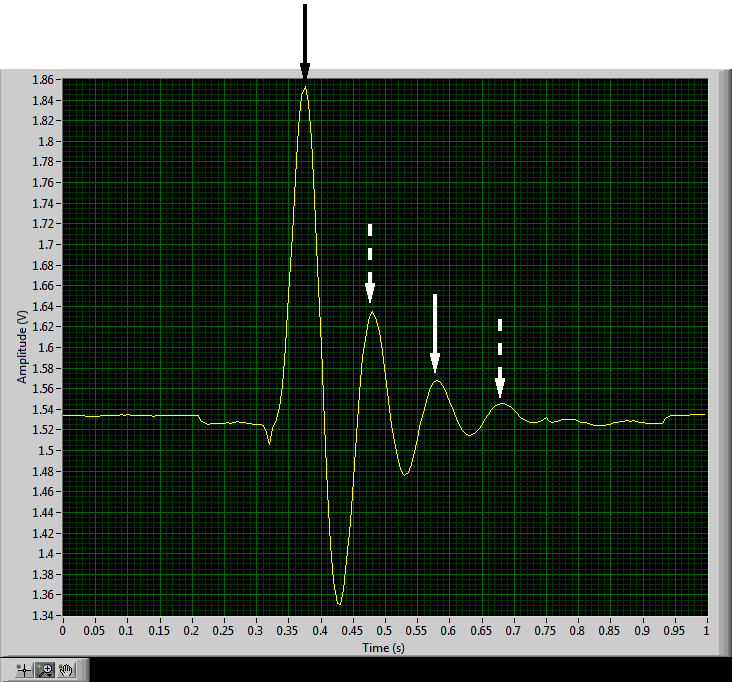
\includegraphics[width=0.5\linewidth]{impresp.png}
\caption{Second-Order System Impulse Response}
\label{fig:impresp}
\end{figure}

\begin{enumerate}

\item The oscillations in Figure~\ref{fig:impresp} occur at the damped
frequency of this system ($\omega_d$).  Is $\omega_d$ greater than or less than
the natural frequency ($\omega_n$) of this system given this impulse response?
Why? [5 points]

$$\omega_d = \omega_n \sqrt{1-\zeta^2}$$

This is an underdamped system, so $\zeta < 1$, meaning that $\omega_d < \omega_n$.  Physically, this should make sense because the damping means that energy is being lost, and that loss mechanism has a finite time constant associated with it that is lower than the natural resonance frequency, causing the downshift (as a function of the damping).

\item Bandwidth:
\begin{itemize}
    \item What is the relative bandwidth (greater or less) of this impulse
response compared to that of a continuous sinusoid oscillating at $\omega_d$?
Why? [5 points]

The bandwidth of the impulse response is greater since that of a continous
sinusoid is a delta function in frequency space and can be considered
infinitely narrow (bandwidth = 0).

    \item What would happen to the bandwidth of this impulse (increase or decrease) if the damping coefficient of this system increased?  Why?  [5 points]

$$2\zeta = \frac{1}{Q}$$

$Q$ is the quality factor, which is inversely proportional to bandwidth, so as $\zeta$ increases, it approaches a critically-damped system, and the quality factor decreases, meaning bandwidth increases.  Physically, an increased damping coefficient means faster decay of the oscillations, and a tighter envelope on that oscillation means a higher bandwidth (Fourier scaling property).

\end{itemize}

\item Draw the block diagram for a circuit that powers an LED with a 0.7 V
threshold voltage on every {\bf other} positive peak of the impulse response
signal above 1.54 V (two solid arrows in Figure~\ref{fig:impresp}) (i.e., use
the impulse response as the input signal into your circuit).  The LED can
remain on until the next temporal positive peak occurs (dashed arrows in
Figure~\ref{fig:impresp}).  Be as detailed as possible in your block diagram.
[15 points]

The following are the key components to {\bf one} of many designs that could work for this problem.

\begin{enumerate}
\item Comparator without hysteresis that transitions at a threshold voltage of 1.54 V.
\item Convert rail voltages of comparator to logical levels (0 \& 5 V).  (There are lots of ways to do this.)
\item Utilize a JK flip flop that will change its output stage on ever negative edge (could be positive if you specific that, depending on the comparator output); this will frequency divide the count by 2, inherently indicating every other comparator transition.
\item Voltage divide (or switch to another source) to provide 0.7 V to the LED and burn the rest of the voltage from the logical high output across a resistor or some other voltage drop.
\end{enumerate}


\end{enumerate}


